% !TeX encoding = UTF-8
%% (requires IEEEtran.cls version 1.7 or later) with an IEEE conference paper.
\documentclass[conference]{IEEEtran}


% *** GRAPHICS RELATED PACKAGES ***
%\usepackage[pdftex]{graphicx}
\usepackage{graphicx}
%\usepackage[dvips]{graphicx}
% to place figures on a fixed position
\usepackage{float}

% *** PDF, URL AND HYPERLINK PACKAGES ***
\usepackage{url}

% correct bad hyphenation here
%\hyphenation{}

\usepackage{xcolor}


\newcommand\note[1]{\textcolor{red}{#1}}
% \renewcommand\note[1]{} % uncomment this line to hide notes

%%%%%%%%%%%%%%%%%%%%%%%%%%%%%%%%%%%%%%%%%%%%%%%%%%%
%%%%%%%%%%%%%%%%%%%%%%%%%%%%%%%%%%%%%%%%%%%%%%%%%%%
%%%%%%%%%%%%%%%%%%%%%%%%%%%%%%%%%%%%%%%%%%%%%%%%%%%
%




\begin{document}


% conference papers do not typically use \thanks and this command
% is locked out in conference mode. If really needed, such as for
% the acknowledgment of grants, issue a \IEEEoverridecommandlockouts
% after \documentclass
% paper title
% can use linebreaks \\ within to get better formatting as desired
\title{Protocol Implementations using FPGAs}
% author names and affiliations
% use a multiple column layout for up to three different
% affiliations
\author{\IEEEauthorblockN{Ferenc Nandor Janky}
\IEEEauthorblockA{Dept. of Telecommunications and MediaInformatics\\Technical University of Budapest\\Budapest, Hungary\\
Email: fecjanky@gmail.com}
}


% make the title area
\maketitle


\begin{abstract}
\boldmath
The handling of connectionless networking protocol messages with low memory utilization could be achieved effectively by using FPGAs. When lower level protocols are implemented in such way, they will provide fast and predictable service characteristics for their upper layer protocols. The perturbation of their software implemented variants such as delay and jitter could be eliminated using the pure hardware implementaion of the operation. One of the key factors of the mentioned side effects is the hosting operating system’s scheduling algorithm.
The purpose of this \dots was to design a generalized approach for implementing protocols using FPGA hardware, and to validate the theory by implementing an application layer protocol using the resulting framework.
The OSI Basic Reference Model is a remarkable guideline as a design basis for setting the boundaries of such framework, because it’s purpose is to provides a common basis for the coordination of standards development for the purpose of systems interconnetion.
As a result of this work the designed framework has been described in VHDL. It follows the basic principles of the OSI reference presenting a general toolkit for handling  PDUs and IDUs beside these features it also provides solutions for other frequently reappearing tasks in the aid of convenient and smoother implementation of various systems interconnecting protocols.
To verify the design a partial implementation of SNMP and various other lower layer protocols have been implemented which was interconnected with with other link, network and transport layer hardware and software products from 3rd party vendors. The conformance testing of the SNMP implementation had been carried out with a couple of network management software.

\end{abstract}


% no keywords

% LaTeX quick ref
%
% \cite{refname} to place citation
%
% \label{label_name} to place a label, which can be reference by \ref{label_name}
%
% new paragraph -> empty line between text
%
% \noindent to not indent paragraphs first line
%
% create list with : \begin{itemize} \end{itemize}
% \begin{itemize
% \renewcommand to renew numbering \labelitemi{--} to select bullet type
% \item item elem 1
% \item item elem2
% \end{itemize}
%
% et alia (et al.) should be emphasized (i.e in italic) with \emph{et al.}
%
% to add figure, htb is placement selector , !overrid internal paramters
%\begin{figure}[!htb]
%    \centering
%    \includegraphics[width=9cm]{FIG.png}
%    \caption{Caption}
%    \label{fig:label}
%\end{figure}
%
% ~ concatenates dynamic text with literals
%
% long dash is --
%
% `is single quoted' , ``is double qouted"


\section{Introduction}\label{sec:Introduction}

some introdcution

\section{Motivation}\label{sec:Motivation}

\section{Related Work}\label{sec:RelatedWork}

here I should introduce some related works

\section{Internal Design}\label{sec:Internal Design}

\begin{figure}[!htb]
    \centering
    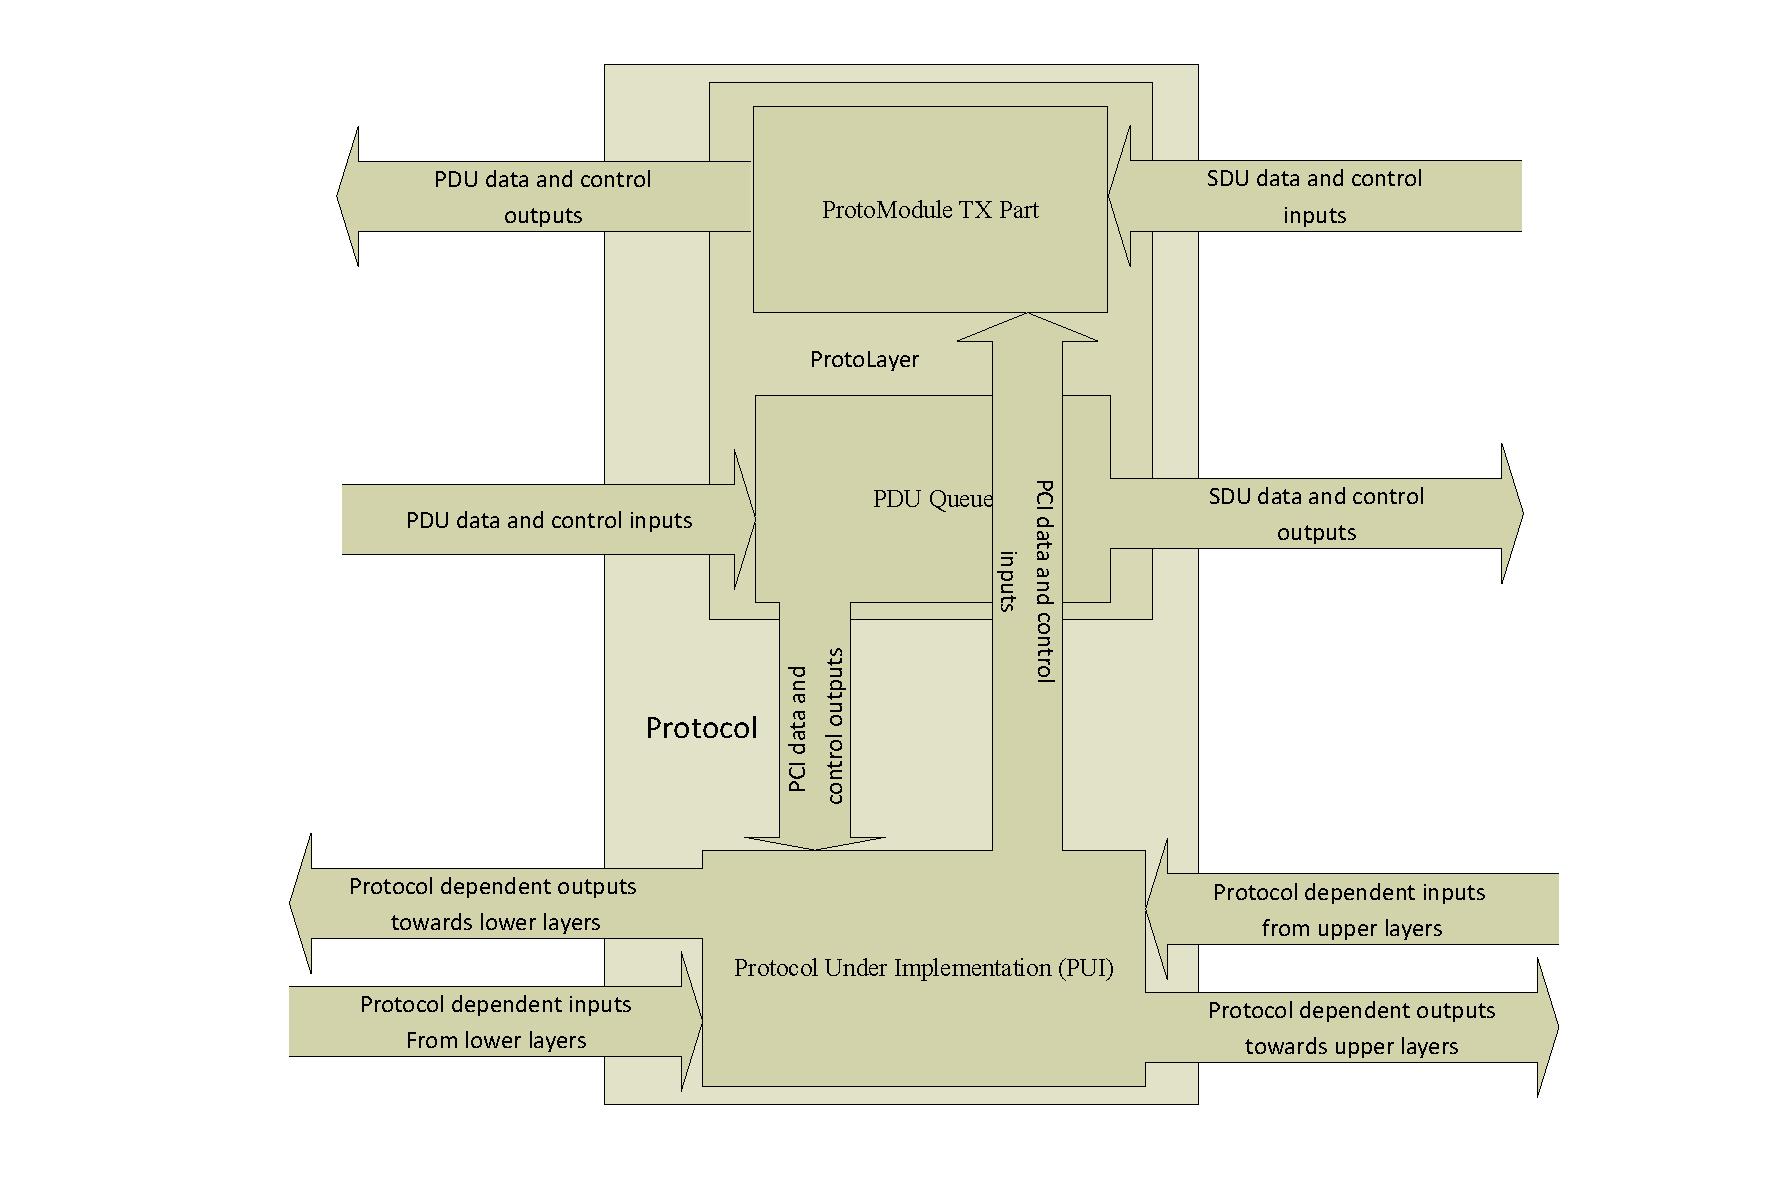
\includegraphics[width=9cm]{figures_raw/protlayer_2.pdf}
    \caption{Schematic drawing of a Protocol layer modul}
    \label{fig:proto_layer_sch}
\end{figure}

\section{Implementation}\label{sec:Implementation}

\section{Verification}


\section{Conclusion}

And summarize with a nice conclusion\cite{Williams_Web_Workload_Characterization_10_Years}

\section{Acknowledgement}
We would like to thank to all of our colleagues and students who contributed to the success of our project


% can use a bibliography generated by BibTeX as a .bbl file
% BibTeX documentation can be easily obtained at:
% http://www.ctan.org/tex-archive/biblio/bibtex/contrib/doc/
% The IEEEtran BibTeX style support page is at:
% http://www.michaelshell.org/tex/ieeetran/bibtex/

\bibliographystyle{IEEEtran}
% argument is your BibTeX string definitions and bibliography database(s)
\bibliography{references}

%
% <OR> manually copy in the resultant .bbl file
% set second argument of \begin to the number of references
% (used to reserve space for the reference number labels box)

%\begin{thebibliography}{1}
%
%\bibitem{IEEEhowto:kopka}
%H.~Kopka and P.~W. Daly, \emph{A Guide to \LaTeX}, 3rd~ed.\hskip 1em plus
% 0.5em minus 0.4em\relax Harlow, England: Addison-Wesley, 1999.
%
% \end{thebibliography}


\end{document}


